\section{The chosen approach}

In order to make things easier and to be able to set tangible milestones, the
challenge is split in two logical problems to be solved, one after the
other, namely:
\begin{enumerate}
	\item{\textbf{Gate center detection:\\}
			The geometric center of the nearest gate in the field of view of the
			drone is to be recognized in real time.
	}
	\item{\textbf{Trajectory planning:\\}
			A trajectory between the current drone position, and the targeted gate
			center is to be generated in real time.
	}
\end{enumerate}

\begin{figure}[h!]
	\centering
	\begin{tikzpicture}[node distance=2cm,-latex]

\pgfdeclarelayer{background}
\pgfdeclarelayer{foreground}
\pgfsetlayers{background,main,foreground}
\tikzstyle{sensor}=[node distance=1.5cm,draw, rectangle,fill=blue!20, text width=2cm,text centered,minimum width=2cm, minimum height=1cm]
\tikzstyle{perc}=[draw, node distance=4cm,draw, rectangle,fill=green!20, text width=2cm,text centered,minimum width=2cm, minimum height=1cm]
\tikzstyle{control}=[draw, node distance=3cm,draw, rectangle,fill=red!20, text width=2cm,text centered,minimum width=2cm, minimum height=3cm]

%% Sensors Nodes 
\node[sensor] (cam) {Camera};
\node[sensor,below of=cam] (imu) {IMU};
\node[sensor,below of=imu] (lidar) {Lidar};
\node[node distance=1cm,above= of cam.west,anchor=west] (sensors) {Sensors};

\begin{pgfonlayer}{background}
    \node[fit=(sensors) (cam) (imu) (lidar), draw,fill=yellow!20] (frame) {}; 
\end{pgfonlayer}

%% Perception Nodes
\node[perc,node distance=4cm,right of=cam] (cnn) {CNN};
\node[perc,right of=cnn] (median) {Median Filter};
\node[node distance=1cm,above= of cnn.west,anchor=west] (perception) {Perception};

\begin{pgfonlayer}{background}
    \node[fit=(perception) (cnn) (median), draw,fill=yellow!20] (frame) {}; 
\end{pgfonlayer}

%% Control Nodes
\node[control,node distance=4.5cm,below of=cnn] (state) {State Machine};
\node[control,right of=state,minimum width=2cm,minimum height=1cm,yshift=1cm] (pid) {PID};
\node[control,right of=pid,minimum width=2cm,minimum height=1cm] (safety) {Safety Mechanism};
\node[control, node distance=2cm,below of=safety,minimum width=4cm,minimum height=1cm] (low) {Low Level Control};
\node[node distance=2cm,above= of state.west,anchor=west] (controller) {Control};

\begin{pgfonlayer}{background}
    \node[fit=(state) (pid) (safety) (low) (controller), draw,fill=yellow!20] (frame) {}; 
\end{pgfonlayer}

%% Connections
\draw[thick] (cam) -- (cnn);
\draw[thick] (cnn) -- (median);
\draw[thick] (lidar.east) -- ++(1cm,0) |- (state);
\draw[thick] (imu) -| ($(pid.north west)!0.33!(pid.north east)$);
\draw[thick] (pid.west) -- ($(state.north east)!0.17!(state.south east)$);
\draw[thick] ($(state.north east)!0.5!(state.south east)$) -| ($(safety.south west)!0.33!(safety.south east)+(0,-0.5cm)$) -- ($(safety.south west)!0.33!(safety.south east)$);
\draw[thick] (pid) -- (safety);
\draw[thick] ($(safety.south west)!0.66!(safety.south east)$) --  ($(low.north west)!0.59!(low.north east)$);
\draw[thick] (median) -- ++(0,-1.5cm) -|($(pid.north west)!0.66!(pid.north east)$);

\end{tikzpicture}

	\caption{Block diagram of the system.}
	\label{fig:block-system}
\end{figure}

~\\The problem is not solved as a whole race, but rather as a trajectory
between a starting point and a gate. This choice of approach is motivated by
the fact that admittedly, if the nearest gate detection is quick and precise,
considering a race as a succession of independent targets to be reached is
theoretically a robust solution that can be applied to any environment, with any
obstacles, and of any length.\\

Firstly, the perception logic is solved with a deep learning algorithm, most
precisely a convolutional neural network. However, it has been seen from
the literature review that collecting a dataset for drone racing can be
tedious, and is rarely variate enough to allow for good generalization of the
learning and application in any given environment. In this work, a
semi-synthetic dataset is generated from background images, to provide an
infinite amount of circuit combinations to train the gate recognition network
(more on that in the following chapter).

In order to detect the closest gate's center, which is the point where the
drone will have to fly through, the problem is simplified so that the output of
the CNN can be directly used by the control logic, without any processing,
except filtering. As shown on figure~\ref{fig:regionproposal}, the input image
is treated as a grid of $N$ windows, numbered from $1$ to $N$, where the
closest gate's center is either inside, or outside. The reason for the indexing
to start at $1$ is justified by the presence of a ``virtual'' window, numbered
$0$, which represents the absence of any gate center in the image. In total,
$N+1$ region proposal windows are considered for the gate center detection
algorithm, event though only $N$ windows actually split the image in a grid.

\begin{figure}[h!]
	\center
	\includegraphics[width=0.7\textwidth]{figure/region_proposal.png}
	\caption[Visual representation of the region proposal grid]{A visual
		representation of the region proposal for the closest gate's center, with
		$N=25$, where the ground truth is annotated in red (window 17), and the gate
		center as the green cross.}
	\label{fig:regionproposal}
\end{figure}

The amount of windows -- minus window $n^{\circ}0$, thus $N$ -- for the region
proposal of the closest gate's center can be adjusted for a more precise
trajectory, but must be a perfect square number to work with the current
implementation, as it greatly simplifies the computation of the ground truth
labels.

Being the main research topic of this thesis, this part is given more time and
focus to deliver a more rigorous and in-depth work.\\

\begin{figure}[h]
	\centering
	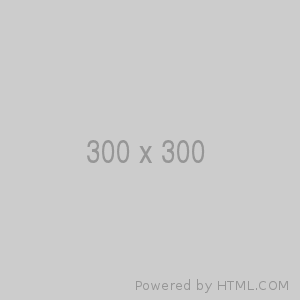
\includegraphics[width=0.5\textwidth]{figure/300x300.png}
	\caption{Block diagram of the perception logic.}
	\label{fig:perception-block}
\end{figure}

Secondly, the control logic is made as simple as can be, since its purpose is
only to verify the hypothesis proposed for the perception. A state machine is
supervising the flight between the two gates, and utilizes a
Proportional-Integral-Derivative controller to output velocity commands to the
lower-level controller implemented by the manufacturer on the UAV.\\

\begin{figure}[h]
	\centering
	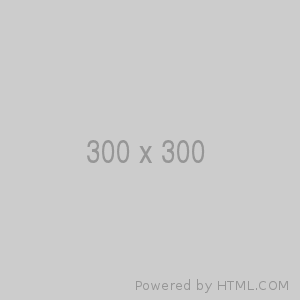
\includegraphics[width=0.5\textwidth]{figure/300x300.png}
	\caption{Block diagram of the control logic.}
	\label{fig:control-block}
\end{figure}

As for the drone itself, the model used to conduct real flight tests is an Intel
Aero, a customizable platform built for developers. It is ready to fly, and
comprises several sensors, namely:

\begin{itemize}
	\item{Intel Atom® x7-Z8750 processor}
	\item{4 GB LPDDR3-1600}
	\item{32 GB eMMC}
	\item{Intel® RealSense™ R200 camera}
		\begin{itemize}
			\item{Depth/infrared: 640x480 resolution at 60FPS}
			\item{RGB: 1080p at 30FPS}
		\end{itemize}
	\item{OmniVision OV8858 8MP RGB camera (front facing)}
		\begin{itemize}
			\item{3264x2448 at 30FPS}
			\item{1080p at 60FPS}
			\item{720p at 90FPS}
			\item{Electronic Image Stabilization}
		\end{itemize}
	\item{OmniVision OV7251 VGA camera, global shutter, monochrome (down facing)}
	\item{GPS and compass}
	\item{Intel® Aero Flight Controller with Dronecode PX4 Autopilot}
\end{itemize}

~\\Since it comes with the Yocto Project~\cite{Yocto} Linux distribution
pre-installed, Ubuntu 16.04 had to be setup first before installing ROS
Kinetic. Unfortunately, the OmniVision OV8858 front facing camera is not
supported on Linux distributions other than the Yocto Project, which means its
high speed video recording feature couldn't be taken advantage of to eliminate
as much motion blur as possible, and instead, the RealSense™ R200 camera is
used. Having a high resolution would be of no interest, since it would only
make the CNN run slower in despite of a negligible gain in accuracy.\\


The solution will be implemented iteratively, by gradually increasing the
complexity of the vision algorithms, such that progress can be made even if the
end goal is too difficult to achieve.\\

The project should attempt to fulfill the following goals:

\begin{itemize}
	\item{Recognize gates in the input image}
	\item{Detect and localize the closest gate's center}
	\item{Evaluate the closest gate's orientation and distance}
	\item{Plan a trajectory for the drone to fly across the gate center}
	\item{Refine the trajectory in real time, for an optimal flight time}
	\item{Make the drone follow that trajectory while adjusting in real time}
\end{itemize}
~\\
However, the following functionalities are out of the scope and will be
discarded:

\begin{itemize}
	\item{Detect any other obstacles in the input image}
	\item{Avoid obstacles that are on the drone's trajectory}
	\item{Map and localize the detected gates in world frame}
	\item{Plan a trajectory of a sequence of gates}
	\item{Apply online learning for adaptive racing}
\end{itemize}
